\documentclass{article}
\usepackage[utf8]{inputenc}
\usepackage[official]{eurosym}
\usepackage{graphicx}
\usepackage[font=small,labelfont=bf]{caption}

\begin{document}

\newcommand{\image}[3]{
\begin{figure}[ht]
\begin{center}
\includegraphics[width=0.75\textwidth]{#1}
\captionof{figure}{#2}
\label{fig:#3}
\end{center}
\end{figure}
}

The Iris dataset was chosen, because of its low dimensionality and its small number of samples, which fulfils the requirement to be contrary to the other selected set and is a good beginning example to classification. Furthermore, it is a very well known dataset, which allows comparison and therefore gives feedback on the performance our results. In general, preprocessing is not mandatory, however since the dataset contains only rational data types, it would be interesting two compare the scaled data versus the non-scaled one. A selection of features is not necessary, since it only consists of four dimensions and already performs quite well.

\subsection{Characteristics}

\begin{itemize}
\item No missing values
\item 3 different target classes
\item Rational quantities, e.g. sepal length, sepal width, petal length, petal width
\item 5 attributes
\item 150 samples
\end{itemize}

Comparing the correlation of the different attributes, \textit{petal width}, \textit{petal length} and \textit{sepal length} are all strong correlated. Only \textit{sepal width} is an exception, which is less and negatively correlated to the others, see Figure \ref{fig:heat}. Thus, sepal width could be a good attribute to distinct between the different classes.

\image{plots/heatmap.png}{Heatmap of the different attrbutes of the Iris dataset}{heat}

\subsection{Characteristics of Classifiers}
A comparison of the different classifiers in sepal width versus sepal length or petal width versus petal length shows, that the class Setosa is the most distinguishable. Concerning the classes Versicolor and Virginica, they are rather unique when comparing them in petal width versus petal length, whereas in sepal width versus sepal length they are not separable. All three classes are uniformly distributed with 50 instances each.

\image

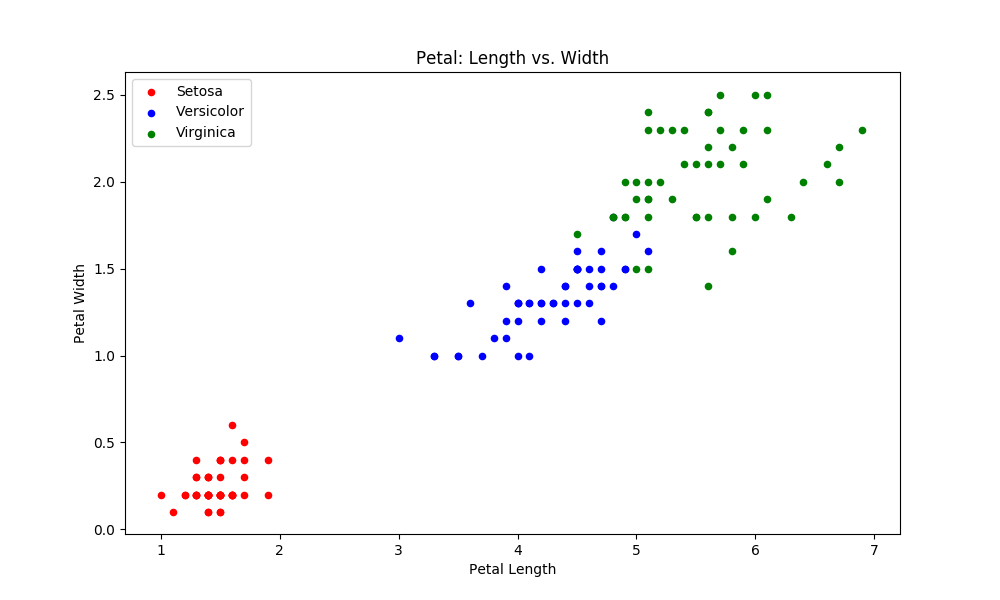
\includegraphics[width=\textwidth]{plots/petal.png}
\captionof{figure}{Comparision of Petal Length versus Petal Width}

\subsection{K Nearest Neighbours Classifier}
For K Nearest Neighbours a \textit{GridSearchCV} was carried out, where especially different \textit{k's} and metrics have been altered. Before that, a more general search has shown, that uniform weights perform better on the Iris dataset. Without preprocessing the best estimator is an Euclidean classifier, where \textit{k} equals 13. Comparing the different metrics, Chebyshev peaks earlier than euclidean, whereas Euclidean generally performed the best and Manhattan the worst. 

\begin{figure}[ht]
\begin{center}
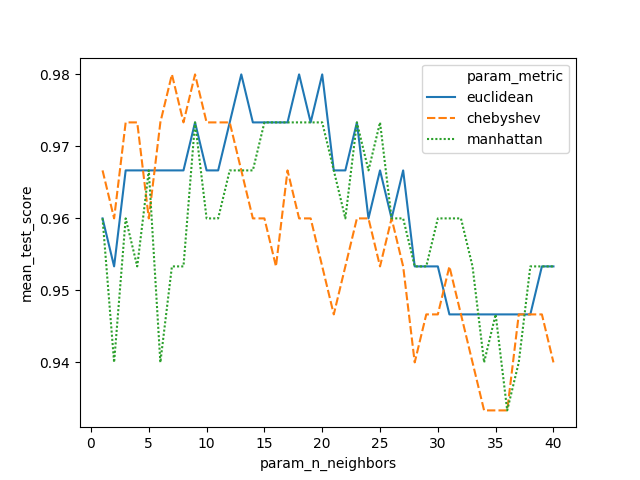
\includegraphics[width=0.75\textwidth]{plots/knn_np_comparision.png}
\captionof{figure}{K Nearest Neighbours with different distance metrics}
\end{center}
\end{figure}

asdfasf

\begin{figure}[ht]
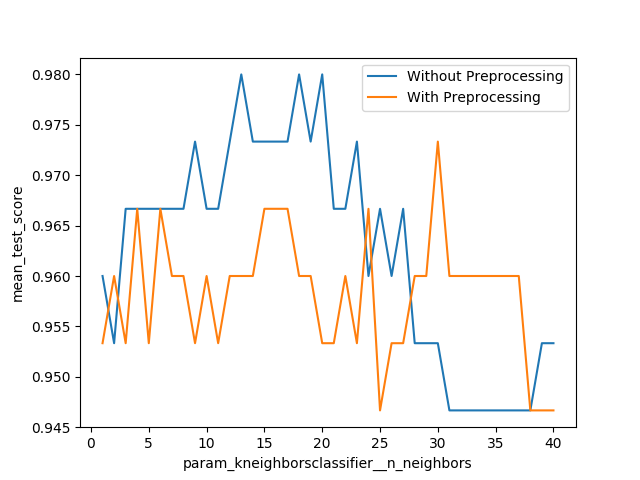
\includegraphics[width=\textwidth]{plots/knn_np_p_comparision.png}
\captionof{figure}{Preprocessing versus No-Preprocessing}
\end{figure}

\subsection{Random Forest Classifier}
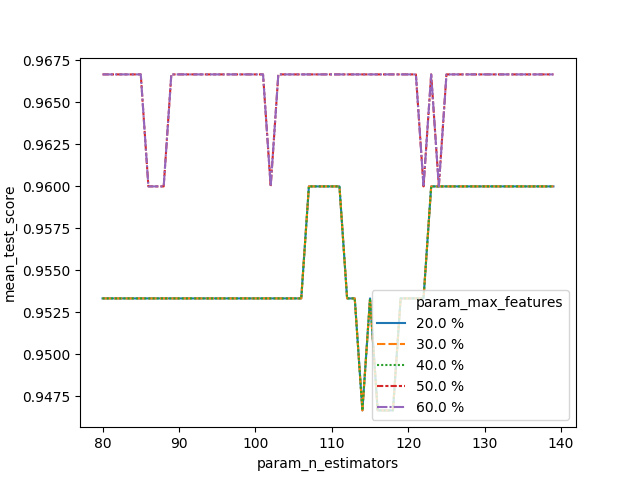
\includegraphics[width=\textwidth]{plots/rf_np_comparision.png}
\captionof{figure}{Comparison of the \textit{max\_features} attribute for different \textit{n\_estimators}}

\subsection{Multi-Layer Perceptron Classifier}
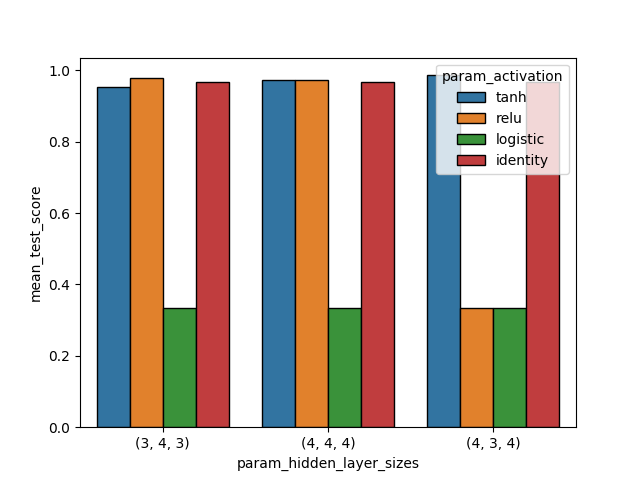
\includegraphics[width=\textwidth]{plots/mlp_np_comparision.png}
\captionof{figure}{Comparison of different models and activation functions}

\subsection{Conclusion}

\begin{table}[h]
\begin{center}
\begin{tabular}{|l|l|l|}
\hline
                       & Preprocessing & No-Preprocessing \\ \hline
KNeighborsClassifier   & 0.9733        & 0.9800           \\ \hline
RandomForestClassifier & 0.9666        & 0.9666           \\ \hline
MLPClassifier          & 0.9666        & 0.9866           \\ \hline
\end{tabular}
\caption{Comparision of accuracy of different techniques with- and without preprocessing}
\end{center}
\end{table}

\begin{table}[h]
\begin{center}
\begin{tabular}{|l|l|l|}
\hline
                       & Holdout & Cross Validation \\ \hline
KNeighborsClassifier   & 0.9333  & 0.9800           \\ \hline
RandomForestClassifier & 0.9666  & 0.9666           \\ \hline
MLPClassifier          & 1.0000  & 0.9866           \\ \hline
\end{tabular}
\caption{Comparision of accuracy of holdout versus cross-validation}
\end{center}
\end{table}

\begin{table}[h]
\begin{center}
\begin{tabular}{|l|l|l|l|l|l|}
\hline
                       & Accuracy & Precision & Recall & F1     & Runtime (sec) \\ \hline
KNeighborsClassifier   & 0.9800   & 0.0.9833  & 0.9799 & 0.9797 & 0.0034        \\ \hline
RandomForestClassifier & 0.9600   & 0.9644    & 0.9600 & 0.9597 & 0.1947        \\ \hline
MLPClassifier          & 0.9800   & 0.9848    & 0.9800 & 0.9793 & 1.5557        \\ \hline
\end{tabular}
\caption{Comparision of different performance metrics and runtimes}
\end{center}
\end{table}

\end{document}